% Welcome! This is the unofficial Integrated Mill Systems Beamer Template.
% IMPORTANT:
% This work, "Integrated Mill Systems Beamer Theme", is a derivative
% of "Umeå University Unofficial Beamer Theme" by Jesper Erixon, CC 4.0 BY.
% (https://www.overleaf.com/latex/templates/umea-university-unofficial-beamer-theme/ptvmzxqzjhcn)
% which is a derivative
% of "University of Udine Unofficial Beamer Theme" by Marco Basaldella, University of Udine, CC 4.0 BY. 
% (https://www.overleaf.com/latex/templates/university-of-udine-unofficial-beamer-theme/zndkgxrjsdzt) 
%
% The main functionality and commands are 
% all credited to Marco Basaldella (and Till Tantau et al. for creating the beamer document class in
% the first place).  
%
% "Integrated Mill Systems Beamer Theme" is licensed under CC 4.0 by Simon Richard.

% Background photo taked by 
% Chris Liverani (https://unsplash.com/@chrisliverani?utm_source=unsplash&utm_medium=referral&utm_content=creditCopyText)
% on Unsplash (https://unsplash.com/s/photos/header-industrial?utm_source=unsplash&utm_medium=referral&utm_content=creditCopyText) 


% Note that [usenames,dvipsnames] is MANDATORY due to compatibility
% issues between tikz and xcolor packages.

\documentclass[usenames,dvipsnames,10pt,aspectratio=169]{beamer} 
% Add option 'aspectratio=169' for 16:9 widescreen 
% Add option  'handout' to ignore animations
% If you have a smaller amount of text, feel free to also try '11pt'! / Jesper

\usepackage[utf8]{inputenc}
\usepackage{verbatim}
\usepackage[nodayofweek,level]{datetime}
\setbeamertemplate{footline}[frame number]
\usetheme{ims}

%%% Bibliography
\usepackage[style=authoryear,backend=biber]{biblatex}
\addbibresource{bibliography.bib}

% Author names in publication list are consistent 
% i.e. name1 surname1, name2 surname2
% See https://tex.stackexchange.com/questions/106914/biblatex-does-not-reverse-the-first-and-last-names-of-the-second-author
\DeclareNameAlias{author}{given-family}

%%% Suppress biblatex annoying warning
\usepackage{silence}
\WarningFilter{biblatex}{Patching footnotes failed}

%%% Some useful commands
% pdf-friendly newline in links
\newcommand{\pdfnewline}{\texorpdfstring{\newline}{ }} 
% Fill the vertical space in a slide (to put text at the bottom)
\newcommand{\framefill}{\vskip0pt plus 1filll}

%%% Additional packages, added by Jesper Erixon
% Use babel to neatly translate 'abstract' etc. to swedish  or other supported language
%\usepackage[swedish]{babel}

%%% Enter additional packages below (or above, I can't stop you)! / Jesper
\renewcommand{\proofname}{\sffamily{Proof}}

%%%%%%%%%%%%%%%%%%%%%%%%%%%%%%%%%%%%%%%%%%%%%%%%%%%%%%%%%%%%%%%%%%%%%%%%%%%%%%%%%%%%%
%%%%%%%%%%%%%%%%%%%%%%%%%%%%%%% YOUR PRESENTATION BELOW %%%%%%%%%%%%%%%%%%%%%%%%%%%%%
%%%%%%%%%%%%%%%%%%%%%%%%%%%%%%%%%%%%%%%%%%%%%%%%%%%%%%%%%%%%%%%%%%%%%%%%%%%%%%%%%%%%%
\newdate{date}{26}{01}{2021}
\title[myTitle]{Tokamak Magnetic Control Simulation: Applications for JT-60SA and ISTTOK Operation.}
\date{\small \displaydate{date}}
%\date[\today]{\small\today}


  
\author[DCorona]{
  Doménica Corona Rivera
  \pdfnewline
 % \texttt{lilia.rivera@tecnico.ulisboa.pt}
}
\institute{Instituto Superior Técnico \newline
Instituto de Plasmas e Fus\~ao Nuclear}


\begin{document}




\begin{frame}
\titlepage
\end{frame}



\begin{frame}{\contentsname}
\tableofcontents
\end{frame}

%%%% New slide 
\section{Magnetic Control}
\begin{frame}{Magnetic Control}

\begin{alertblock}{Warning}
You can ignore this slide if you're \textbf{not} working with Overleaf.
\end{alertblock}

 \begin{figure}[htbp]
	\centering
	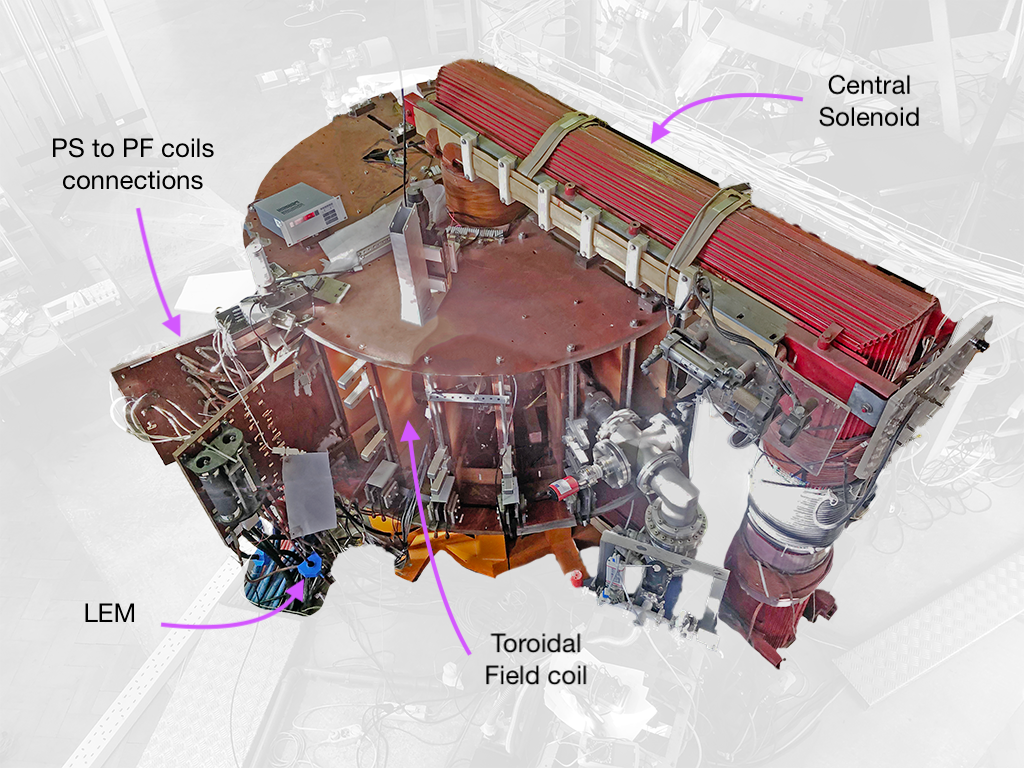
\includegraphics[width=0.38\textwidth]{Figures/TopISTTOK.png}
	\caption{\label{TopISTTOK} ISTTOK top view in 2020,   main elements are indicated with magenta  lines.}
\end{figure}

\end{frame}

\begin{frame}[fragile]
\frametitle{Compiling}

\begin{alertblock}{Warning}
You can ignore this slide if you \textbf{are} working with Overleaf.
\end{alertblock}

To compile this deck you'll need the \texttt{biber} package. Probably your \TeX editor already supports it; if not, you will easily find online the instructions to install it.

\vskip 0.5cm

If you're not using an editor, you can compile this presentation using the command line by running:

\begin{verbatim}
$ pdflatex main.tex
$ biber main.bcf
$ pdflatex main.tex
$ pdflatex main.tex
\end{verbatim}


\end{frame}

\section{Plasma Control Systems}
\begin{frame}{Plasma Control Systems}

\end{frame}

\section{Control Techniques}
\begin{frame}{Control Techniques}
    
\end{frame}



\section{Contributions}
\begin{frame}{Contributions}
    
\end{frame}


\framepic[0.5]{graphics/bkground}{
	\vfill
    \begin{flushright}
    \textcolor{black}{\textbf{It will probably take half a century but nuclear fusion may become practicable and  a limitless source of energy}}
    \end{flushright}	
}

\section{Colors}

\begin{frame}{Colors}

For this template we defined two colors:
\begin{itemize}
\item \textcolor{white}{\marker[IMSBlue]{\texttt{IMSBlue}}}
\item \textcolor{white}{\marker[IMSOrange]{\texttt{IMSOrange}}}
\end{itemize}

\vskip 0.5cm

You can use these colors as you want in your presentation. For example, you can \textbf{\textcolor{IMSOrange}{color the text in orange}} by writing \texttt{\textbackslash textcolor\{IMSOrange\}\{my green text\}}.

\vskip 0.5cm

We also redefined many of the most common \LaTeX{} and Beamer commands, like \texttt{itemize}, \texttt{block}, etc. You will see samples of these commands in the following slides.

\end{frame}

\section{Blocks}

\begin{frame} 
\frametitle{This is a page with a title and a subtitle} 
\framesubtitle{And also some blocks.} 
\begin{block}{Goal of the mission}
Shoot in the Death Star's exhaust port and destroy it before it can fire on the Rebel base.
\end{block} 
\begin{alertblock}{Take care!}
TIE Fighters may chase you while approaching the target.
\end{alertblock} 
\begin{exampleblock}{Use the force you must}
Remember your training with Obi-Wan, and use the Force to make the perfect shot.
\end{exampleblock} 

\end{frame}

\section{Enumerates, itemizes and description}

\subsection{Enumerates and itemizes}


\begin{frame}{Enumerates and itemizes}

This is an example of \texttt{itemize}.
\begin{itemize}
	\item A long time ago in a galaxy far, far away...
\end{itemize}
And this is an example of \texttt{enumerate}.

\begin{enumerate} 
  \item Go to the Death Star.
  \item Find the exhaust port.
  \item Make the perfect shot.
  \item Become a hero.
\end{enumerate}
\end{frame}

\subsection{Description}

\begin{frame}[fragile]
\frametitle{Description}
This is an example of \texttt{description}.

\begin{description}
\item<2->[Vader] \emph{I am} your father.
\item<1->[Luke] No. No! That's not true! \textbf{That's impossible!}
\end{description}

\begin{uncoverenv}<3>
  \vskip 0.5cm
  And while we're here, let's have a look to \texttt{verbatim} as well, to see how we made items appear in arbitrary order:
  \vskip 0.5cm
  \begin{verbatim}
\begin{description}
  \item<2->[This is the first item - appears after] one
  \item<1->[This is the second item - appears first] two
\end{description}
  \end{verbatim}
\end{uncoverenv}

\end{frame}

\section{Maths}

\begin{frame}{Maths}
A formula will look like this: 
\begin{center}
 $x^2 + y^2 = z^2$
\end{center}

You can number equations as well:
\begin{equation}
1+1=2
\end{equation}

\begin{equation}
1+1=2 \tag{custom label!}
\end{equation}

\vskip 0.5cm

If you want to use the sans serif math fonts, or use a serif font for the main text, just go to \texttt{beamerfontthemeims.sty} and select the indicated font option. 

\end{frame}

\begin{frame}{Theorems}

The usual \texttt{theorem}, \texttt{corollary}, \texttt{definition}, \texttt{definitions}, \texttt{fact}, \texttt{example} and \texttt{examples} blocks are available as well.

\begin{theorem}
There exists an infinite set.
\end{theorem}
\begin{proof}
This follows from the axiom of infinity.
\end{proof}
\begin{example}[Natural Numbers]
The set of natural numbers is infinite. 
\end{example}

\end{frame}

\section{Other blocks}

\begin{frame}{Other blocks}

Here we display examples of \texttt{abstract}, \texttt{verse}, \texttt{quotation}, and \texttt{quote}.

\vskip 0.5cm

\begin{abstract}
This is an abstract.
\end{abstract}
\begin{verse}
This is a verse.
\end{verse}
\begin{quotation}
This is a quotation.

\raggedleft -Han Solo
\end{quotation}
\begin{quote}
A quote this is.

\raggedleft -Yoda
\end{quote}

\end{frame}

\section{Bibliography and Publications}
\begin{frame}[fragile]
\frametitle{Bibliography}

You can cite an article
\begin{itemize}
\item normally using \texttt{\textbackslash cite}, e.g.: (\cite{article1})
\item or display the full citation using \texttt{\textbackslash fullcite}, e.g.:  \fullcite{article1} \\\vspace{0.4cm}

\textit{(n.d.) stands for "no date". \texttt{year=\{A long time ago...\}} is not a date that should be specified in \texttt{bibliography} anyway.}
\end{itemize}

\vskip 0.5cm
Look at the code of the following slide to see how to automatically split the bibliography on many slides. You can also use \texttt{\textbackslash nocite\{*\}} to display the non-cited publications as well.

\end{frame}

\begin{frame}[t,allowframebreaks]
\frametitle{Bibliography}

\nocite{*} % will display the non-cited publications as well. Useful for a publication list.

\printbibliography

\end{frame}

\section{Bonus Commands}

\begin{frame}[fragile]
\frametitle{Framecard}

You can display a frame with a colored background and a huge text in the center using the command \texttt{\textbackslash framecard}.
\vskip 0.5cm 
For example, you can write:
\begin{verbatim}
\framecard{A SECTION\\TITLE}
\end{verbatim}

This will display a frame with a blue background and the phrase "A SECTION TITLE" in the center. You can also use a custom color with \texttt{\textbackslash framecard}:
\begin{verbatim}
\framecard{A SECTION TITLE}
\framecard[IMSOrange]{A SECTION TITLE\\
WITH A CUSTOM COLOR}
\end{verbatim}
You can see the results of the commands above in the following slides.

\end{frame}

\framecard{A SECTION TITLE}
\framecard[IMSOrange]{A SECTION TITLE\\\vspace{4pt}WITH A CUSTOM COLOR}

\begin{frame}[fragile]
\frametitle{Framepic}

You can display a frame with a background image using the command \texttt{\textbackslash framepic}. The image will be \textbf{adapted vertically} to fit the the frame. 

For example, you can write:
\begin{verbatim}
\framepic{graphics/darth}{
	\framefill
    \textcolor{white}{Luke,\\I am your supervisor}
    \vskip 0.5cm
}
\end{verbatim}

Alternatively, to make the background 50\% transparent, you can write \texttt{\textbackslash framepic[0.5]\{graphics/darth\}...}



You can see the results of the commands above in the following slides.

\end{frame}


\framepic{graphics/darth}{
	\framefill
    \textcolor{white}{Luke,\\I am your supervisor}
    \vskip 0.5cm
}

\framepic[0.5]{graphics/bkground}{
	\vfill
    \begin{flushright}
    \textcolor{IMSBlue}{\textbf{Ending}}
    \end{flushright}	
}



\end{document}